\section{MÔ HÌNH ĐỘNG HỌC PHÂN TỬ CHẤT KHÍ}
\subsection{LÝ THUYẾT TRỌNG TÂM}
\subsubsection{Chuyển động Brown}
\begin{boxdn}
	Chuyển động Brown là chuyển động hỗn loạn không ngừng, không theo quy luật, có quỹ đạo là những đường gấp khúc bất kì của các hạt nhẹ trong chất lỏng và chất khí. Chuyển động Brown chứng tỏ các phân tử chất khí chuyển động hỗn loạn, không ngừng. Nhiệt độ càng cao, các phân tử chuyển động càng nhanh.
\end{boxdn}
\begin{center}
	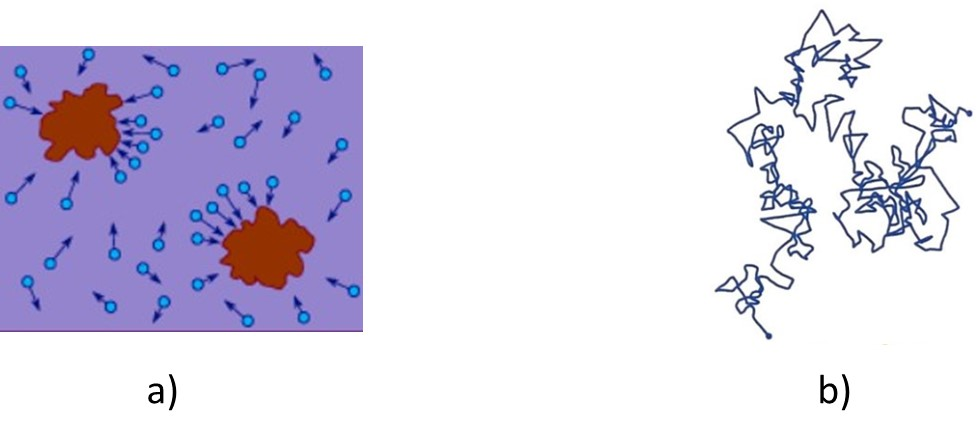
\includegraphics[width=0.5\linewidth]{figs/VN12-Y24-PH-SYL-009-1}
	\captionof{figure}{a) Va chạm của các phân tử nước lên hạt phấn hoa, b) Minh hoạ quỹ đạo gấp khúc của một hạt phấn hoa trong nước. }
\end{center}
\subsubsection{Chất khí}
\paragraph{Tính chất của chất khí}
\begin{boxdn}
	Chất khí có một số tính chất sau:
	\begin{itemize}
		\item Chất khí có hình dạng và thể tích của vật chứa nó.
		\item Chất khí có khối lượng riêng nhỏ hơn nhiều so với chất lỏng và chất rắn.
		\item Chất khí dễ bị nén.
		\item Chất khí gây ra áp suất lên thành bình chứa nó. Khi nhiệt độ tăng, áp suất khí tác dụng lên thành bình tăng.
	\end{itemize}
\end{boxdn}
\paragraph{Lượng chất}
\begin{boxdn}
	Mol là lượng chất trong đó chứa số phân tử (hoặc nguyên tử) bằng 
	$$N_A\approx\SI{6.02E23}{\mole^{-1}}$$
	$N_A$ được gọi là số Avogadro (số phân tử trong 1 mol chất).\\
	Khối lượng mol của một chất là khối lượng của $\SI{1}{\mole}$ chất đó, được kí hiệu là $M$.\\
	Nếu một mẫu chất có khối lượng $m$, chứa $N$ phân tử thì số mol $n$ của mẫu chất đó được xác định:
	$$n=\dfrac{N}{N_A}=\dfrac{m}{M}.$$
\end{boxdn}
\subsubsection{Mô hình động học phân tử chất khí}
\begin{boxdn}
	Nội dung mô hình động học phân tử chất khí gồm các ý chính như sau:
	\begin{itemize}
		\item Chất khí gồm tập hợp rất nhiều các phân tử có kích thước rất nhỏ so với khoảng cách trung bình giữa chúng.
		\item Các phân tử khí luôn chuyển động hỗn loạn, không ngừng và được gọi là chuyển động nhiệt. Nhiệt độ càng cao, các phân tử khí chuyển động càng nhanh.
		\item Trong quá trình chuyển động, các phân tử khí va chạm với thành bình chứa, gây ra áp suất lên thành bình.
	\end{itemize}
\end{boxdn}
\begin{center}
	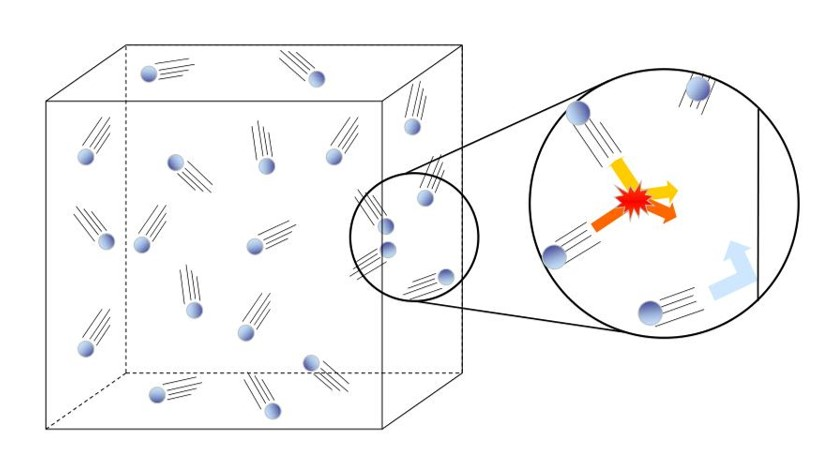
\includegraphics[width=0.4\linewidth]{figs/VN12-Y24-PH-SYL-009-2}
	\captionof{figure}{Các phân tử va chạm vào nhau và va chạm vào thành bình trong quá trình chuyển động nhiệt.}
\end{center}
\subsubsection{Khí lí tưởng}
\begin{boxdn}
	Khí lí tưởng có các đặc điểm sau:
	\begin{enumerate}[label=\arabic*.]
		\item Các phân tử khí được coi là các \textit{chất điểm}, không tương tác với nhau khi chưa va chạm.
		\item Các phân tử khí tương tác khi va chạm với nhau và va chạm với thành bình. Các va chạm này là va chạm \textit{hoàn toàn đàn hồi}.
	\end{enumerate}
\end{boxdn}
\begin{luuy}
	Mô hình khí lí tưởng đơn giản hơn khí thực (khí tồn tại trong thực tế) nhưng vẫn phản ánh được các đặc điểm cơ bản của khí này.
\end{luuy}
\subsection{VÍ DỤ MINH HOẠ}
\begin{dang}{Phân tích mô hình Brown, nêu được các phân tử trong chất khí chuyển động hỗn loạn.}
	\end{dang}
	\begin{vd}
Khi quan sát tia nắng mặt trời chiếu qua cửa sổ vào trong phòng, ta có thể thấy các hạt bụi trong ánh nắng chuyển động không ngừng. Chuyển động này có phải là chuyển động Brown không? Tại sao?
	\loigiai{Chuyển động của các hạt bụi trong trường hợp này không thể coi là chuyển động Brown vì chuyển động chủ yếu của các hạt bụi lúc bấy giờ là chuyển động theo dòng khí do hiện tượng đối lưu.
			}
	\end{vd}

\begin{dang}{Vận dụng được thuyết động học phân tử chất khí}
\end{dang}
\begin{vd}
Trong quá trình bơm xe đạp, khi lốp xe đã gần căng, càng về cuối của mỗi lần bơm thì ta càng thấy khó nén piston xuống. Hãy giải thích hiện tượng trên.
\loigiai{Càng về cuối quá trình bơm săm xe đạp, săm xe đã căng và khó tăng thể tích chứa khí bên trong. Trong khi đó, sau mỗi lần bơm thì số phân tử khí bên trong săm tăng lên đáng kể và làm tăng mật độ phân tử khí bên trong. \\
		Theo thuyết động học phân tử chất khí, khi mật độ phân tử khí bên trong săm tăng thì số va chạm của các phân tử khí lên thành săm và piston tăng. Do đó, áp suất khí tác động lên piston tăng và làm cho piston khó nén xuống hơn.
	}

\end{vd}
% ==================================================================
\begin{vd}
Một phân tử oxygen đang chuyển động qua tâm một bình cầu có đường kính $\SI{0.20}{\meter}$. Tốc độ của phân tử là $\SI{400}{\meter/\second}$. Ước tính số lần phân tử này va chạm vào thành bình chứa trong mỗi giây. Coi rằng tốc độ của phân tử là không đổi.
\loigiai{Trong điều kiện lý tưởng, xem như phân tử oxygen chuyển động thẳng và không bị đổi hướng do va chạm với các phân tử khí khác, tốc độ của phân tử là không đổi và va chạm của phân tử khí với thành bình là tuyệt đối đàn hồi. Ban đầu phân tử khí này chuyển động qua tâm bình cầu nên khi chạm vào thành bình, phân tử khí sẽ bật ngược trở lại với tốc độ như cũ và cũng đi qua tâm bình cầu.\\
		Khoảng thời gian giữa 2 lần liên tiếp phân tử khí va chạm với thành bình:
		$$T=\dfrac{2R}{v}=\dfrac{\SI{0.2}{\meter}}{\SI{400}{\meter/\second}}=\SI{5E-4}{\second}.$$
		Số lần phân tử khí này va chạm vào thành bình trong mỗi giây:
		$$f=\dfrac{1}{T}=2000.$$
	}
\end{vd}
\subsection{BÀI TẬP TRẮC NGHIỆM}
\Opensolutionfile{ans}[ans/G12Y24B8TN]
% ===================================================================
\begin{ex}
	Tính chất nào sau đây \textbf{không phải} là tính chất của chất khí?
	\choice
	{\True Có hình dạng và thể tích riêng.}
	{Có các phân tử chuyển động hỗn loạn không ngừng.}
	{Có thể nén được dễ dàng.}
	{Có khối lượng riêng nhỏ hơn so với chất rắn và chất lỏng.}
	\loigiai{}
\end{ex}
% ===================================================================
\begin{ex}
	Chọn phương án \textbf{sai}. Số Avogadro là
	\choice
	{số phân tử (hay nguyên tử) có trong $\SI{22.4}{\text{lít}}$ khí ở điều kiện tiêu chuẩn $\left(\SI{0}{\celsius}, \SI{1}{atm}\right)$.}
	{số phân tử (hay nguyên tử) có trong 1 mol chất.}
	{\True số phân tử (hay nguyên tử) có trong 1 đơn vị khối lượng chất.}
	{số nguyên tử có trong $\SI{12}{\gram}$ $\ce{^{12}C}$.}
	\loigiai{}
\end{ex}
% ===================================================================
\begin{ex}
Gọi $\xsi{M}{(\gram/\mole)}$ là khối lượng mol nguyên tử, $N_\text{A}$ là số Avogadro. Biểu thức xác định số phân tử hay nguyên tử chứa trong $\xsi{m}{(\gram)}$ của chất đó là	
	\choice
	{$N=MmN_\text{A}$.}
	{$N=\dfrac{MN_\text{A}}{m}$.}
	{\True $N=\dfrac{mN_\text{A}}{M}$.}
	{$N=\dfrac{N_\text{A}}{mM}$.}
	\loigiai{}
\end{ex}
% ===================================================================
\begin{ex}
Điền vào chỗ trống.\\
Chất khí trong đó các phân tử được coi là \dots và chỉ tương tác khi \dots được gọi là khí lí tưởng.	
	\choice
	{\True chất điểm; va chạm.}
	{vật rắn; va chạm.}
	{chất điểm; ở gần nhau.}
	{vật rắn; ở gần nhau.}
	\loigiai{}
\end{ex}
% ===================================================================
\begin{ex}
	Nhận xét nào sau đây về các phân tử khí lí tưởng là \textbf{không đúng}?
	\choice
	{Có thể tích riêng không đáng kể.}
	{Có lực tương tác không đáng kể khi không va chạm.}
	{\True Có khối lượng không đáng kể.}
	{Có vận tốc càng lớn khi nhiệt độ phân tử càng cao.}
	\loigiai{}
\end{ex}
% ===================================================================
\begin{ex}
Chọn câu \textbf{sai}. Số Avogadro có giá trị bằng	
	\choice
	{số nguyên tử chứa trong $\SI{4}{\gram}$ helium.}
	{\True số phân tử chứa trong $\SI{16}{\gram}$ oxygen.}
	{số phân tử chứa trong $\SI{18}{\gram}$ nước lỏng.}
	{số nguyên tử chứa trong $\SI{22.4}{\liter}$ khí trơ ở $\SI{0}{\celsius}$ và áp suất $\SI{1}{atm}$.}
	\loigiai{}
\end{ex}
% ===================================================================
\begin{ex}
Một bình kín chứa $N=\SI{3.01E23}{}$ phân tử khí helium. Khối lượng helium chứa trong bình là	
	\choice
	{$\SI{0.5}{\gram}$.}
	{$\SI{1}{\gram}$.}
	{\True $\SI{2}{\gram}$.}
	{$\SI{4}{\gram}$.}
	\loigiai{}
\end{ex}
% ===================================================================
\begin{ex}
	Cho biết khối lượng riêng của không khí ở điều kiện tiêu chuẩn là $\SI{1.29}{\kilogram/\meter^3}$. Coi không khí như một chất khí thuần nhất, khối lượng mol của không khí là
	\choice
	{$\SI{0.041}{\kilogram/\mole}$.}
	{\True $\SI{0.029}{\kilogram/\mole}$.}
	{$\SI{0.023}{\kilogram/\mole}$.}
	{$\SI{0.026}{\kilogram/\mole}$.}
	\loigiai{$$\rho=\dfrac{m}{V}=\dfrac{m}{n\cdot\left(\SI{22.4E-3}{\meter^3}\right)}\Rightarrow M=\dfrac{m}{n}=\SI{0.029}{\kilogram/\mole}.$$}
\end{ex}
\Closesolutionfile{ans}
\subsection{TRẮC NGHIỆM ĐÚNG/SAI}
\setcounter{ex}{0}
% ===================================================================
\begin{ex}
	Nhận định các phát biểu sau về đặc điểm của chuyển động Brown.
	\begin{enumerate}[label=\alph*)]
	\item Chuyển động Brown tuân theo một số quy luật nhất định.
	\item Quỹ đạo của chuyển động Brown là những đường gấp khúc.
	\item Chuyển động Brown là chuyển động của các hạt nhẹ trong chất rắn, lỏng, khí.
	\item Nhiệt độ càng cao thì các phân tử khí chuyển động càng hỗn loạn.
\end{enumerate}
	\loigiai{\begin{enumerate}[label=\alph*)]
			\item Sai. Chuyển động Brown không theo quy luật.
			\item Đúng.
			\item Sai. Chuyển động Brown là chuyển động của các hạt nhẹ trong chất lỏng và chất khí.
			\item Đúng.
		\end{enumerate}
	}
\end{ex}
% ===================================================================
\begin{ex}
	Nhận định các phát biểu sau về nội dung thuyết động học phân tử chất khí.
	\begin{enumerate}[label=\alph*)]
		\item Chất khí gồm tập hợp nhiều các phân tử dao động nhiệt quanh các vị trí cân bằng của chúng.
		\item Nhiệt độ càng cao thì các phân tử khí chuyển động nhiệt càng nhanh.
		\item Kích thước các phân tử rất nhỏ so với khoảng cách trung bình giữa chúng.
		\item Áp suất khí được tạo ra bởi sự va chạm giữa các phân tử khí với nhau.
	\end{enumerate}
	\loigiai{\begin{enumerate}[label=\alph*)]
			\item Sai. Các phân tử khí chuyển động hỗn loạn, không ngừng.
			\item Đúng.
			\item Đúng.
			\item Sai. Sự va chạm của các phân tử khí với thành bình gây ra áp suất lên thành bình.
		\end{enumerate}
	}
\end{ex}
% ===================================================================
\begin{ex}
	Nhận định các phát biểu sau đây về đặc điểm của khí lí tưởng
	\begin{enumerate}[label=\alph*)]
		\item Các phân tử khí được coi là chất điểm nên người ta có thể bỏ qua khối lượng các phân tử khí.
		\item Thể tích khối khí bằng thể tích bình chứa trừ đi thể tích riêng của các phân tử.
		\item Các phân tử khí chỉ tương tác với nhau khi va chạm.
		\item Nội năng của khối khí bằng tổng động năng chuyển động nhiệt của các phân tử khí và chỉ phụ thuộc vào nhiệt độ.
	\end{enumerate}
	
	\loigiai{\begin{enumerate}[label=\alph*)]
			\item Sai. Các phân tử khí được coi là chất điểm nên người ta có thể bỏ qua kích thước các phân tử khí.
			\item Sai. Thể tích khối khí bằng thể tích bình chứa.
			\item Đúng.
			\item Đúng.
		\end{enumerate}
	}
\end{ex}
% ===================================================================
\begin{ex}
	Một người xịt nước hoa ở đầu phòng thì người ở cuối phòng vẫn nghe được mùi hương của nước hoa.
	\begin{enumerate}[label=\alph*)]
		\item Hiện tượng trên được gọi là sự khuếch tán.
		\item Các phân tử nước hoa chuyển động thành dòng từ đầu phòng sang cuối phòng chỉ nhờ vào đối lưu.
		\item Hiện tượng trên chứng tỏ nhiệt độ ở đầu phòng cao hơn nhiệt độ ở cuối phòng.
		\item Nhiệt độ trong phòng càng cao thì người ở cuối phòng càng sớm nhận ra mùi nước hoa.
	\end{enumerate}
	
	\loigiai{\begin{enumerate}[label=\alph*)]
			\item Đúng.
			\item Sai. Sự dao động nhiệt của các phân tử khí và phân tử nước hoa làm cho chúng khuếch tán vào nhau.
			\item Sai. Các phân tử khí chuyển động hỗn loạn, không ngừng về mọi phía nên không thể khẳng định được nhiệt độ nơi nào cao hơn.
			\item Đúng. Nhiệt độ càng cao, các phân tử chuyển động càng nhanh làm tốc độ khuếch tán diễn ra càng nhanh.
		\end{enumerate}
	}
\end{ex}
\subsection{BÀI TẬP TỰ LUẬN}
\setcounter{ex}{0}
% ===================================================================
\begin{ex}
	Mùi hôi từ các bãi rác thải là một vấn nạn đối với cư dân sống xung quanh. Khi thời tiết càng nắng nóng thì mùi hôi bốc ra càng nồng nặc và càng bay xa (ngay cả trong điều kiện không có gió). Dựa vào thuyết động học phân tử chất khí, hãy giải thích điều này và đề xuất biện pháp hạn chế tình trạng trên.
	\loigiai{Thời tiết càng nóng thì quá trình phân huỷ các chất hữu cơ diễn ra càng nhanh và sinh ra nhiều khí có mùi hôi như: $\ce{H_2S}, \ce{NH_3}, \ce{CH_4}, \ce{SO_2},\dots$. Bên cạnh đó, nhiệt độ càng cao thì các phân tử khí chuyển động nhiệt càng nhanh, do đó các phân tử khí này càng dễ khuếch tán vào không khí và bay đi xa hơn.\\
		Biện pháp hạn chế: Thường xuyên thu gom, xử lý rác thải, nâng cao ý thức cộng đồng.
	}
\end{ex}
% ===================================================================
\begin{ex}
Đun một nồi nước trên bếp, khi nước sôi nắp nồi thường bị đẩy lên. Hãy giải thích điều này.
	
	\loigiai{Khi đun nước đến nhiệt độ sôi, nước sẽ bay hơi tạo thành hơi nước. Bên cạnh đó, nhiệt độ càng cao làm cho các phân tử khí và hơi nước trong nồi chuyển động càng nhanh. Sự gia tăng mật độ khí và tốc độ chuyển động nhiệt của các phân tử khí và hơi nước trong nồi làm gia tăng số lượt va chạm của các phân tử khí lên nắp nồi $\rightarrow$ tăng áp suất khí tác dụng lên nắp và làm nắp bị đẩy lên.
	}
\end{ex}
% ===================================================================
\begin{ex}
	Xác định số phân tử chứa trong
	\begin{enumerate}[label=\alph*)]
		\item $\SI{0.2}{\kilogram}$ nước.
		\item $\SI{1}{\kilogram}$ không khí nếu như không khí có $\SI{22}{\percent}$ là khí $\ce{O_2}$ và $\SI{78}{\percent}$ là khí $\ce{N_2}$.
	\end{enumerate}
	\loigiai{\begin{enumerate}[label=\alph*)]
			\item $N=\dfrac{m}{M_{\ce{H_2O}}}\cdot N_\text{A}\approx\SI{6.68E24}{\text{phân tử}}.$
			\item $N=\SI{22}{\percent}\cdot\dfrac{m}{M_{\ce{O_2}}}\cdot N_\text{A}+\SI{78}{\percent}\cdot\dfrac{m}{M_{\ce{N_2}}}\cdot N_\text{A}\approx\SI{2.1E25}{\text{phân tử}}.$
		\end{enumerate}
	}
\end{ex}
% ===================================================================
\begin{ex}
	Coi Trái Đất là một khối cầu bán kính $\SI{6400}{\kilo\meter}$, nếu lấy toàn bộ số phân tử nước trong $\SI{1.0}{\gram}$ hơi nước trải đều trên bề mặt Trái Đất thì mỗi mét vuông trên bề mặt Trái Đất có bao nhiêu phân tử nước? Biết khối lượng mol của phân tử nước khoảng $\SI{18}{\gram/\mole}$.
	\loigiai{$$\eta=\dfrac{N}{S}=\dfrac{\dfrac{m}{M}N_\text{A}}{4\pi R^2}=\SI{64.98E6}{\text{phân tử}/\meter^2}.$$}
\end{ex}